\documentclass[11pt]{article}
\usepackage[scaled=0.92]{helvet}
\usepackage{geometry}
\geometry{letterpaper,tmargin=1in,bmargin=1in,lmargin=1in,rmargin=1in}
\usepackage[parfill]{parskip} % Activate to begin paragraphs with an empty line rather than an indent %\usepackage{graphicx}
\usepackage{amsmath,amssymb, mathrsfs, dsfont, stackrel}
\usepackage{tabularx}
\usepackage[font=footnotesize,labelfont=bf]{caption}
\usepackage{graphicx}
\usepackage{xcolor}
%\usepackage[linkbordercolor ={1 1 1} ]{hyperref}
%\usepackage[sf]{titlesec}
\usepackage{natbib}
\usepackage{../../Tianpei_Report}
%\usepackage{appendix}
%\usepackage{algorithm}
%\usepackage{algorithmic}

%\renewcommand{\algorithmicrequire}{\textbf{Input:}}
%\renewcommand{\algorithmicensure}{\textbf{Output:}}



\begin{document}
\title{Lecture 5: Causal Estimation}
\author{ Tianpei Xie}
\date{Sep. 22nd., 2022 }
\maketitle
\tableofcontents
\newpage
\allowdisplaybreaks
\section{Recall what we learned}
\begin{itemize}
\item Given a populuation, we can compute the \underline{\emph{\textbf{average treatment effect (ATE)}}}, or, \emph{average causal effect (ACE)} \citep{imbens2015causal,  rosenbaum2017observation,  neal2020introduction}  by taking an average over the ITEs:
\begin{align}
\tau &:=  \E{}{Y_i(1) - Y_i(0)} =  \E{}{Y(1)} -\E{}{Y(0)} \label{eqn: ATE}
\end{align} where the average is over the individuals $i$ if $Y_i(t)$ is deterministic. If $Y_i(t)$ is random, the average is also over any other randomness.

\item We have the following assumptions that are commonly used
\begin{itemize}
\item \begin{assumption} (\textbf{Ignorability / Exchangeability}) \citep{neal2020introduction}
\begin{align}
(Y(1), Y(0)) \indep T  \label{eqn: Ignorability}
\end{align}
\end{assumption}

\item \begin{assumption} (\textbf{Conditional Exchangeability / Unconfoundedness}) \citep{neal2020introduction}
\begin{align}
(Y(1), Y(0)) \indep T \;|\; X \label{eqn: conditional_exchangeablity}
\end{align} 
\end{assumption}

\item \begin{assumption} (\textbf{Positivity / Overlap / Common Support})  \citep{neal2020introduction}\\
For all values of covariates $x$ present in the population of interest (i.e. $x$ such that $P(X = x) > 0$),
\begin{align}
0 < P(T=1 | X = x) < 1 \label{eqn: positive}
\end{align}
\end{assumption} 

\item \begin{assumption}(\textbf{No Interference}) \citep{neal2020introduction}\\
\begin{align}
Y_{i}(t_1, \ldots, t_i, \ldots, t_n) &= Y_{i}(t_i) \label{eqn: no_interference}
\end{align}
\end{assumption}

\item \begin{assumption}(\textbf{Consistency}) \citep{neal2020introduction}\\
If the treatment is $T$, then the observed outcome $Y$ is the potential outcome under treatment $T$. Formally,
\begin{align}
T=t &\Rightarrow Y = Y(t) \label{eqn: consistency}
\end{align}
We could write this equivalently as follow:
\begin{align}
Y = Y(T) \label{eqn: consistency2}
\end{align}
\end{assumption}

\item \textbf{\emph{Stable unit-treatment value assumption (SUTVA)}} is satisfied if unit (individual) $i$'s outcome is simply a \textbf{function} of unit $i$'s treatment. Therefore, SUTVA is a combination of consistency and no interference (and also \emph{\textbf{deterministic}} potential outcomes). 
\end{itemize}

\item \begin{theorem}(\textbf{Adjustment Formula})  \citep{neal2020introduction}\\
Given the assumptions of \textbf{unconfoundedness}, \textbf{positivity}, \textbf{consistency}, and \textbf{no interference}, we can identify the average treatment effect:
\begin{align*}
\tau= \E{}{Y(1) - Y(0)} &= \E{X}{ \E{}{Y \,|T=1,\,X }- \E{}{Y \,|T=0, \, X}}  
\end{align*}
\end{theorem}

\item  \begin{definition} (\textbf{\emph{Structural causal models (SCMs})}) \citep{peters2017elements}\\
A \textbf{SCM} $\mathfrak{C}:= (S, P_{\mb{N}})$ with graph $\cG=(\cV, \cE)$ consists of a collection $S$ of $d$ \emph{\textbf{(structural) assignments}}:
\begin{align}
X_{s} &:= f_{s}(X_{\pi(s)}, N_s), \quad s=1,\ldots, d \label{eqn: scm}
\end{align} where $X_{\pi(s)}$ are called \textbf{parents} of $X_s$; and a joint distribution $P_{\mb{N}} = \prod_{s=1}^{d}P_{N_{s}}$ over the noise variables, which we require to be \underline{\emph{\textbf{jointly independent}}}.

The $\cG=(\cV, \cE)$ of a SCM is obtained by creating one vertex for each $X_s$ and drawing \textbf{directed edges} from each parent in $X_{\pi(s)}$ to $X_s$, that is, from each variable $X_k$ occurring on the right-hand side of equation \eqref{eqn: scm} to $X_s$. $\cG$ is a  \textbf{directed acyclic graph (DAG)}.

We sometimes call the elements of $X_{\pi(s)}$ not only parents but also \underline{\textbf{\emph{direct causes}}} of $X_s$, and we call $X_s$ a \underline{\textbf{\emph{direct effect}}} of each of its direct causes. SCMs are also called (\textbf{\emph{nonlinear}}) \textbf{\emph{SEMs}}.
\end{definition}

\begin{figure}
\begin{minipage}[t]{1\linewidth}
  \centering
  \centerline{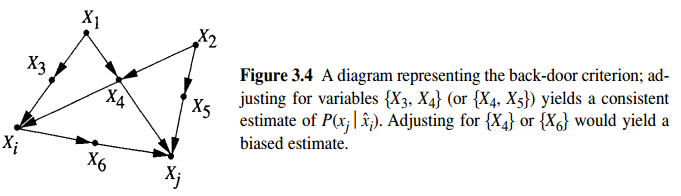
\includegraphics[scale = 0.6]{backdoor.png}}
\end{minipage}
\caption{\footnotesize{\textbf{The back-door adjustment  \citep{pearl2000causal}}}}
\label{fig: backdoor}
\end{figure}

\item 
\begin{definition}(\textbf{\emph{Back-Door}}) \citep{pearl2000causal}\\
A set of variables $Z$ satisfies the \emph{\textbf{back-door criterion}} relative to an \emph{\textbf{ordered}} pair of variables $(X_i \rightarrow X_j)$ in a DAG $\cG$ if:
\begin{enumerate}
\item \emph{\textbf{no}} node in $Z$ is a \emph{\textbf{descendant}} of $X_i$; and
\item $Z$ \emph{\textbf{blocks every path}} between $X_i$ and $X_j$ that contains an arrow \textbf{\emph{into}} $X_i$.
\end{enumerate}
Similarly, if $X$ and $Y$ are two \textbf{disjoint} subsets of nodes in $\cG$, then $Z$ is said to satisfy \textbf{\emph{the back-door criterion}} relative to $(X, Y)$ if it satisfies the criterion relative to \emph{any pair} $(X_i, X_j)$ such that $X_i \in X$ and $X_j \in Y$.
\end{definition} 

\item  Satisfying the back-door criterion makes $Z$ a \emph{\textbf{sufficient adjustment set}}. The main insight of the graphical approach to covariate adjustment is that the adjustment set must \textbf{block all \emph{noncausal} paths} \textbf{without blocking} any \emph{\textbf{causal}} paths between $X$ and $Y$. 

\item \begin{theorem} (\textbf{Back-Door Adjustment}) \citep{pearl2000causal, neal2020introduction}\\
If a set of variables $Z$ satisfies the back-door criterion relative to $(X, Y)$, then the causal effect of $X$ on $Y$ is \textbf{identifiable} and is given by the formula
\begin{align}
P(y\,|\, do(x)) &= \sum_{z}P(y\,|\,x,  z)P(z) \label{eqn: back_door_adjustment}
\end{align}
\end{theorem} To see why this works we need to know that $P(z| do(x)) = P(z)$ since by back-door criterion, $Z$ has no descendant of $X$. Also $P(y\,|\,do(x),  z) = P(y\,|\,x,  z)$ since $Z$ blocks all paths from $X$ to $Y$, so by modularity 

\item \begin{definition} (\emph{\textbf{Front-Door}}) \citep{pearl2000causal}\\
A set of variables $M$ is said to satisfy the \emph{\textbf{front-door criterion}} relative to an \emph{\textbf{ordered}} pair of variables $(T, Y)$ if:
\begin{enumerate}
\item $M$ \textbf{intercepts} \textbf{all} directed paths from $T$ to $Y$;
\item there is \emph{\textbf{no unblocked back-door path}} from $T$ to $M$; and
\item \emph{\textbf{all back-door paths}} from $M$ to $Y$ are \emph{\textbf{blocked}} by $T$.
\end{enumerate}
\end{definition} 

\item  A set of variables $M$ \emph{\textbf{completely mediates}} the effect of $T$ on $Y$ if all causal (directed) paths from $T$ to $Y$ go through $M$. If $M$ satisfies the front-door criterion, $M$ is a set of complete mediators.

\item \begin{theorem}(\textbf{Front-Door Adjustment}) \citep{pearl2000causal, neal2020introduction}\\
If $M$ satisfies the front-door criterion relative to $(T, Y)$ and if $P(t, m) > 0$, then the causal
effect of $T$ on $Y$ is \textbf{identifiable} and is given by the formula
\begin{align}
P(y | \, do(t)) &=  \sum_{m}P(m|\, t)\,\sum_{t'}P(y|\, m, t')\,\,P(t')
\end{align}
\end{theorem}

\item 
\begin{proposition}(\textbf{Rules of do Calculus})\citep{pearl2000causal}  \\
Let $\cG$ be the directed acyclic graph associated with a causal model as defined in \eqref{eqn: scm_1}, \eqref{eqn: scm_2}, and let $P(\cdot)$ stand for the probability distribution induced by that model. For any \textbf{disjoint} subsets of variables $X$, $Y$, $Z$, and $W$, we have the following rules.
\begin{enumerate}
\item (\textbf{Insertion/deletion of observations}):
\begin{align}
p(y| \hat{x}, z, w)&= p(y| \hat{x},  w) \quad \text{if }(Y \indep Z | X, W)_{\widehat{\cG}_{X}} \label{eqn: do_del_ob}
\end{align} where $\hat{x} := do(X=x)$ and $\widehat{\cG}_{X}$ is induced sub-graph under intervention $\hat{x}$.

\item (\textbf{Action/observation exchange}):
\begin{align}
p(y| \hat{x}, \hat{z}, w)&= p(y| \hat{x}, z, w) \quad \text{if }(Y \indep Z | X, W)_{\widehat{\cG}_{X, Z}}  \label{eqn: do_exch_act_ob}
\end{align} where $\widehat{\cG}_{X,Z}$ is induced sub-graph under intervention $\hat{x}, \hat{z}$.

\item  (\textbf{Insertion/deletion of actions}):
\begin{align}
p(y| \hat{x}, \hat{z}, w)&= p(y| \hat{x},  w) \quad \text{if }(Y \indep Z | X, W)_{\widehat{\cG}_{X, Z(W)}} \label{eqn: do_del_act}
\end{align} where $Z(W)$ is the set of $Z$-nodes that are \textbf{not ancestors} of any $W$-node in $\widehat{\cG}_{X}$.
\end{enumerate}
\end{proposition}
\end{itemize}

\newpage
\section{Conditional Outcome Modeling (COM)}
\subsection{Basic concepts}
\begin{figure}
\begin{minipage}[t]{1\linewidth}
  \centering
  \centerline{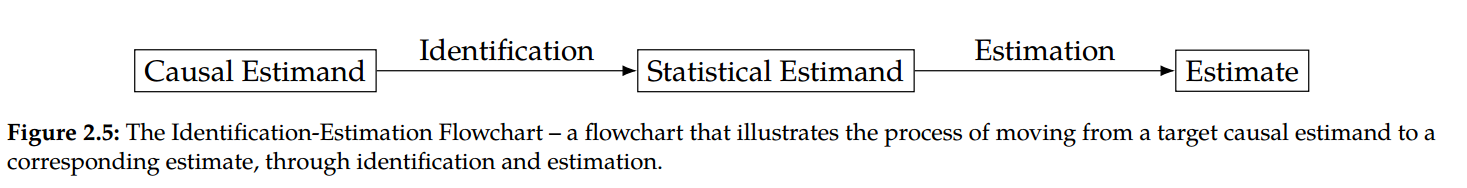
\includegraphics[scale = 0.35]{idt_est.png}}
\end{minipage}
\caption{\footnotesize{\textbf{The basic process of identification and estimation in causal inference.  \citep{neal2020introduction}}}}
\label{fig: idt_est}
\end{figure}
\begin{itemize}
\item From Adjustment Formula, we see that 
\begin{align*}
\tau= \E{}{Y(1) - Y(0)} &= \E{\mb{X}}{ \E{}{Y \,|T=1,\,\mb{X} }- \E{}{Y \,|T=0, \, \mb{X}}}  
\end{align*}

On the left hand side, it is a causal estimand and on the right hand side, it is a statistical estimand. 

\item To estimate the ATE $\tau$, we need to fit a model for $ \E{}{Y \,|T,\, \mb{X} }$ and then approximate $\E{\mb{X}}{\delta_{\mb{X}}}$, with an empirical mean over the $n$ data
points. 
\begin{align}
\delta_{X} := \mu(1, \mb{x}) - \mu(0, \mb{x}) &=  \E{}{Y \,|T=1,\,\mb{X} }- \E{}{Y \,|T=0, \, \mb{X}} \label{eqn: cond_outcome} \\
\text{where }\mu(t, \mb{x})&:= \E{}{Y \,|T=t,\,\mb{X} = \mb{x} } \nonumber
\end{align}

Here the estimated model $\hat{\mu}(t, \mb{x})$ is called \underline{\textbf{\emph{conditional outcome model (COM)}}}. Then the estimated ATE is
\begin{align}
\hat{\tau} &= \sum_{i=1}^{n}\paren{\hat{\mu}(1, \mb{x}_i) - \hat{\mu}(0, \mb{x}_i)} \label{eqn: cond_outcome_est_ate}
\end{align} We will refer to estimators that take this form as \emph{\textbf{conditional outcome model (COM) estimators}}.

\item For each individual covariate, we may be interested in the \emph{\textbf{conditional average treatment effect (CATE)}} $\tau(\mb{x})$: 
\begin{align}
\tau(\mb{x})= \E{}{Y(1) - Y(0) \,|\, \mb{X} = \mb{x}} \label{eqn: cate}
\end{align} The $X$ that is conditioned on does not need to consist of all of the observed covariates, but this is often the case when people refer to CATEs. For each individual subject, we call that \emph{\textbf{individualized average treatment effects (IATEs)}}.

\item When we are interested in the CATE, we can split the covariate set as $W\cup X$, where $X$ are observed covariates, then the COM model 
\begin{align*}
\mu(t,  \mb{w}, \mb{x}) &:= \E{}{Y |\, T=t,\,W=\mb{w},\, \mb{X}=\mb{x}} 
\end{align*}
Then CATE estimator is
\begin{align}
\hat{\tau}(\mb{x}) &= \sum_{i \in \set{i: \mb{x}_i = \mb{x}}}\paren{\hat{\mu}(1,\mb{w}_i,  \mb{x}) - \hat{\mu}(0, \mb{w}_i,  \mb{x})} \label{eqn: cond_outcome_est_cate}
\end{align} and the IATE estimator is 
\begin{align}
\hat{\tau}(\mb{x}_i) &=\hat{\mu}(1,\mb{w}_i,  \mb{x}_i) - \hat{\mu}(0, \mb{w}_i,  \mb{x}_i) \label{eqn: cond_outcome_est_iate}
\end{align} Even, though IATEs are different from ITEs ($\tau(\mb{x}_i) \neq \tau_i$), if we really want to give estimates for ITEs, it is relatively common to take this estimator
as our estimator of the ITE $\tau_i$ as well.

\item COM estimators have many different names in the literature. For example, they are often called \textbf{\emph{G-computation estimators}}, \emph{\textbf{parametric G-formula}}, or \textit{\textbf{standardization}} in epidemiology and biostatistics \citep{imbens2015causal}. Because we are fitting a \emph{single statistical model} for $\mu$ here, "COM estimator" is sometimes referred to as an “\emph{S-learner},” where the “S” stands for “single.”
\end{itemize}


\subsection{Grouped Conditional Outcome Modeling (GCOM)}
\begin{itemize}
\item COM above train a single model $\mu(t, \mb{x}) = \E{}{Y \,|T=t,\,\mb{X} = \mb{x} }$ based on $(\mb{X}, T, Y)$, where $T$ is \emph{\textbf{1-dimensional}} and $\mb{X}$ is \emph{multi-dimensional}. It is likely that models would ignore variable $T$ and focus on the rest of covariates.  But $T$ is only thing changing between two terms. This would result in an ATE estimate of zero.

\item The solution is to train \textbf{two} models, one for treatment group and one for control group: 
\begin{align}
\mu_1(\mb{x}):= \E{}{Y\,|\,T=1, \, \mb{X}=\mb{x}},\quad  \mu_0(\mb{x}):= \E{}{Y\,|\,T=0, \, \mb{X}=\mb{x}}  \label{eqn: grouped_cond_outcome}
\end{align} Using two separate models for the values of treatment ensures that $T$ cannot be ignored. These models are called \underline{\emph{\textbf{grouped conditional
outcome model (GCOM)}}}. 

\item The \emph{\textbf{grouped conditional outcome model (GCOM) estimator}} for ATE is
\begin{align}
\hat{\tau} &= \sum_{i=1}^{n}\paren{\hat{\mu}_1(\mb{x}_i) - \hat{\mu}_0(\mb{x}_i)} \label{eqn: grouped_cond_outcome_est_ate}
\end{align}

\item Similarly, for CATE, 
\begin{align}
\hat{\tau}(\mb{x}) &= \sum_{i \in \set{i: \mb{x}_i = \mb{x}}}\paren{\hat{\mu}_1(\mb{w}_i,  \mb{x}) - \hat{\mu}_0(\mb{w}_i,  \mb{x})} \label{eqn: grouped_cond_outcome_est_cate}
\end{align}

\item The GCOM may fix the zero estimate for ATE but it has a \textbf{major drawback}: each model is trained on \textbf{a sub-population of data} (i.e. treatment group or control group). This cause a significant drop in \textbf{\emph{data efficiency}}.

\end{itemize}

\section{Increasing Data Efficiency: TARNet and X-learning}
\begin{itemize}
\item One way to mitigate the data efficiency issue is to learn a \textbf{\emph{treatment-agnostic representation (TAR)}} of covariates $\mb{X}$, using all of the data while still forcing the model to not ignore $T$ by \textbf{branching} into \emph{\textbf{two heads}} for the different values of $T$.  In other words, \emph{\textbf{TARNet}} \citep{shalit2017estimating} uses the knowledge we have about $T$ (as a uniquely important variable) in its architecture.  See details in \citep{neal2020introduction}.

\item Another solution is to use \underline{\emph{\textbf{X-learners}}} \citep{kunzel2019metalearners, neal2020introduction}, which is neither COM or GCOM. These models use all of the data for both models that are part of the estimators.

\item Note that the CATE has \underline{\emph{\textbf{Observational-Counterfactual Decomposition}}} \citep{neal2020introduction}.
\begin{align}
\E{}{Y(1) - Y(0)\,|\,\mb{X} = \mb{x}} &= e(\mb{x}) \tau_1(\mb{x}) +(1-e(\mb{x}))\tau_0(\mb{x})  \nonumber \\
 \tau_1(\mb{x}) &= \E{}{Y\,| \, T=1,\,\mb{X} = \mb{x}} - \E{}{Y(0) | T=1,\,\mb{X} = \mb{x}} \label{eqn: x_learner_iate_1} \\
 &:= \E{}{Y - \mu_0(\mb{X})\,|\,T=1, \, \mb{X}=\mb{x}} \nonumber\\
  \tau_0(\mb{x}) &=\E{}{Y(1) \,|\, T=0,\,\mb{X} = \mb{x}}  - \E{}{Y \,|\, T=0,\,\mb{X} = \mb{x}}\label{eqn: x_learner_iate_0} \\
 &:=  \E{}{\mu_1(\mb{X}) - Y\,|\,T=0,\,\mb{X} = \mb{x}} \nonumber
\end{align} where $e(\mb{x}) = P(T=1 | \mb{X}=\mb{x})$ is the \emph{\textbf{propensity score}}. $\tau_1(\mb{x})$ and $\tau_0(\mb{x})$ are causal estimands.

\item Like GCOM, X-learner first estimates the \emph{\textbf{conditional potential outcomes}}
\begin{align}
\mu_1(\mb{x}) &= \E{}{Y(1) | \mb{X} = \mb{x}} = \E{}{Y |\, do(T=1),\,\mb{X} = \mb{x}} , \label{eqn: x_learner_counter_1}\\
 \mu_0(\mb{x}) &= \E{}{Y(0) | \mb{X} = \mb{x}} =  \E{}{Y |\, do(T=0),\, \mb{X} = \mb{x}}   \label{eqn: x_learner_counter_0}
\end{align} using
\begin{align*}
\hat{\mu}_1(\mb{x}) &= \Em{model}{Y |\, T=1,\, \mb{X} = \mb{x}} \\
\hat{\mu}_0(\mb{x}) &= \Em{model}{Y |\, T=0,\, \mb{X} = \mb{x}}.
\end{align*} The main difference is that $\hat{\mu}_1(\mb{x})$ and $\hat{\mu}_0(\mb{x})$ are served as a \underline{\textbf{\emph{counterfactual term}}} in the target, where they are used to train treatment responses $\hat{\tau}_0(\mb{x})$ and $\hat{\tau}_1(\mb{x})$ in \emph{\textbf{alternative}} group as compared to their training set .

There are three steps to X-learning:
\begin{enumerate}
\item Learning \textbf{two models} $\hat{\mu}_0(\mb{x})$ and $\hat{\mu}_1(\mb{x})$ from using \emph{control group data} and \emph{treatment group data}, respectively. 

\item Then we define the \emph{\textbf{target}} in the treatment and control group using the estimated ITE
\begin{align}
\hat{\tau}_{1,i} &= Y_i(1) - \hat{\mu}_0(\mb{x}_i)  \label{eqn: x_learner_target_1}\\
\hat{\tau}_{0,i} &=  \hat{\mu}_1(\mb{x}_i)  - Y_i(0) \label{eqn: x_learner_target_0}
\end{align} Here, $\hat{\tau}_{1,i}$ is estimated using the \textbf{\emph{treatment group outcomes}} and the \emph{\textbf{imputed counterfactual}} in $\hat{\mu}_0(\mb{x}_i)$, which was learned from the \emph{\textbf{control group data}}. Similarly, $\hat{\tau}_{0,i}$ is estimated using the \emph{\textbf{control group outcomes}} and the \underline{\emph{\textbf{imputed counterfactual}}} $\hat{\mu}_1(\mb{x}_i)$ using \emph{\textbf{treatment group data}}. 

This method is called \textbf{$X$-learning} since the observational and counterfactual terms are arranged in "$X$" shaped in \eqref{eqn: x_learner_target_1} and \eqref{eqn: x_learner_target_0}. 

%Importantly, each treatment group ITE estimate $\hat{\tau}_{1,i}$ uses both \emph{\textbf{treatment group data}} (the \emph{observed potential outcome under treatment}), and \emph{\textbf{control group data}} (e.g. in $\hat{\mu}_0$).  and $\hat{\tau}_{0,i}$ 

We can fit model $\hat{\tau}_1(\mb{x}_i)$ using data $\set{(\mb{x}_{i}, \hat{\tau}_{1,i}), i\in \cT}$ from the \textbf{\emph{treatment group}} subjects. Similarly, we fit model $\hat{\tau}_{0}(\mb{x}_i)$  using data $\set{(\mb{x}_{j}, \hat{\tau}_{0,j}), j \in  \cC}$  from the  \textbf{\emph{control group}} subjects.

\item Finally, the estimated CATE is
\begin{align}
\hat{\tau}(\mb{x}) &= \hat{e}(\mb{x}) \hat{\tau}_1(\mb{x}) + (1 - \hat{e}(\mb{x})) \hat{\tau}_{0}(\mb{x}) \label{eqn: x_learner_ate}
\end{align} where $\hat{e}(\mb{x}) \in [0, 1]$ is an estimate of propensity score $e(\mb{x})$.
\end{enumerate}
\end{itemize}
\section{Inverse Probability Weighting (IPW)}
\begin{figure}
\begin{minipage}[t]{0.5\linewidth}
  \centering
  \centerline{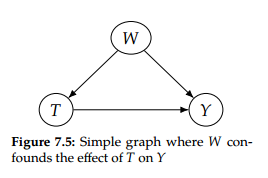
\includegraphics[scale = 0.6]{IPW_1.png}}
  \vspace{-5pt}
  \centerline{(a)}
\end{minipage}
\begin{minipage}[t]{0.5\linewidth}
  \centering
  \centerline{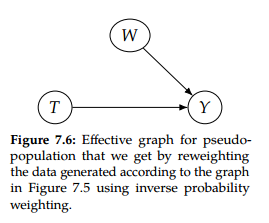
\includegraphics[scale = 0.6]{IPW_2.png}}
  \vspace{-5pt}
  \centerline{(b)}
\end{minipage}
\caption{\footnotesize{\textbf{The effective causal graph for pseudo-population generated via inverse probability weighting}}}
\label{fig: ipw}
\end{figure}

\begin{itemize}
\item \underline{\emph{\textbf{Matching perspective}}}: Remember during matching with propensity score, we match subjects in treatment and control group with the same propensity score. Suppose there is a subset of subjects  in both groups whose propensity scores are matched. Instead of choosing only a pair of them for matching, we can \textbf{choose all of them as matched} and \textbf{\emph{downweight}} the contribution of each sample \emph{\textbf{uniformly}}. There are in total $P(T=1 | \mb{w}_{r}) \times N_{\mb{w}_r}$ matched treated subjects. So we need to reweighting these subjects by the \emph{\textbf{inverse probability of treatment}} $\frac{1}{P(T=1 | \mb{w}_{r})}$. Similarly, the matched control subjects is reweighted by $\frac{1}{P(T=0 | \mb{w}_{r})}$. 

By reweighting, each matched sample contributed the same, which is equivalent to selecting just one pair of samples from matched subsets.

\item \underline{\emph{\textbf{Oversampling perspective}}}:  In an \emph{observational study}, certain groups may be \underline{\textbf{\emph{oversampled}}} relative to the hypothetical sample from a \emph{\textbf{randomized trial}} due to existence of \textbf{confounder} $\mb{W}$. 

Specifically, in Figure \ref{fig: ipw} (a), the group of treated data with confounder $\mb{W} = \mb{w}$ are sampled according to the propensity score $P(T=1|\,\mb{w})$, which is different from the hypothetical sampling probability $P(T=1)$ under randomized trial. $P(T=1|\,\mb{w}) \neq P(T=1)$.

We can \emph{\textbf{resample}} the population with probability $\frac{1}{P(T=1|\,\mb{W})}$ for the treatment group and $\frac{1}{P(T=0|\,\mb{W})}$ for the control group. By this way, we get a \underline{\emph{\textbf{pseudo-population}}} where $P(T=1|\,\mb{W}) = P(T=1)$ or equals some constant; the important part is that we make $T$ independent of $\mb{W}$. In this pseudo-population, the treatment group and control group are \emph{balanced}, i.e. \emph{\textbf{everyone is equally likely to be treated}}. See Figure \ref{fig: ipw} (b). Large weights from IPW means that the given subject was likely to be treated, given their covariates, \emph{but wasn't}.

\item We can derive the \underline{\emph{\textbf{Inverse Probability Weighting (IPW)} estimator}}
\begin{align}
\E{}{Y(t)} &= \E{\mb{W},Y}{\frac{\ind{T=t}\,Y}{P(T=t\,|\,\mb{W}\,)}} \label{eqn: ipw_po_est}
\end{align} This is a \emph{\textbf{causal identification equation}}, where the left hand side is a causal estimand and the right hand side is a statistical estimand.
The proof follows from the adjustment formula 
\begin{align*}
\E{}{Y(t)} &= \E{\mb{W}}{\E{}{Y \,|\, t, \mb{W}}}\\
&=\sum_{\mb{w}} \sum_{y}y\, P(y |\, t, \mb{w})P(\mb{w})  \\
&= \sum_{\mb{w}} \sum_{y}y\, \frac{P(y |\, t, \mb{w})P(t\,|\,\mb{w}\,)P(\mb{w}) }{P(t\,|\,\mb{w}\,)}\\
&= \sum_{\mb{w}} \sum_{y} y\, P(y, t, \mb{w})\, \frac{1}{P(t\,|\,\mb{w}\,)}\\
&= \sum_{\mb{w}} \E{}{\ind{\mb{W}=\mb{w} \land T=t} Y} \,\frac{1}{P(t\,|\,\mb{w}\,)}\\
&= \E{\mb{W}, Y}{\frac{\ind{T=t} Y}{P(t\,|\,\mb{W}\,)}} \qed
\end{align*}

\item Assuming binary treatment (and \emph{\textbf{exchangeablity}} and \emph{\textbf{positivity}} so that $1/P(T=t\,|\,\mb{W}\,)$ exists), the following identification equation for the ATE follows from \eqref{eqn: ipw_po_est}:
\begin{align}
\tau= \E{}{Y(1) - Y(0)} &=\E{\mb{W}, Y}{\frac{\ind{T=1}\,Y}{e(\mb{W})}} - \E{\mb{W}, Y}{\frac{\ind{T=0}\,Y}{1 - e(\mb{W})}}. \label{eqn: ipw_ate}
\end{align}
We have the sample IPW estimator for ATE: 
\begin{align}
\hat{\tau}&= \frac{1}{n}\sum_{i}\paren{\frac{\ind{T_i=1}\,y_i}{\hat{e}(\mb{w}_i)} - \frac{\ind{T_i=0}\,y_i}{1 - \hat{e}(\mb{w}_i)}} \nonumber \\
&= \frac{1}{n_{T}}\sum_{i: T_i = 1}\frac{y_i}{\hat{e}(\mb{w}_i)} - \frac{1}{n_{C}}\sum_{i: T_i = 0} \frac{y_i}{1 - \hat{e}(\mb{w}_i)}, \label{eqn: ipw_ate_est}
\end{align} where $n_T$ and $n_C$ are number of treated subjects and control subjects, respectively.

\item We can also find the IPW estimator of CATE:
\begin{align}
\hat{\tau}(\mb{x})&=  \frac{1}{n_{\mb{x}}}\sum_{i: \mb{x}_i = \mb{x}}\paren{\frac{\ind{T_i=1}\,y_i}{\hat{e}(\mb{w}_i)} - \frac{\ind{T_i=0}\,y_i}{1 - \hat{e}(\mb{w}_i)}}, \label{eqn: ipw_cate_est}
\end{align} where $n_{\mb{x}}$ is the number of data points with $\mb{x}_i = \mb{x}$. 

However, with limited sample size, this estimator may suffer high variance issue.

\item We want to \underline{\textbf{trim the tails}} on the \textbf{propensity score distribution} so that the IPWs would \textbf{not} be \textbf{too high} and the \textbf{positivity assumption} is not violated. But it would change the distribution.  We can also \underline{\textbf{truncate the scores}}, which increase bias but decrease variance.

\item We may \textbf{normalize} the inverse probability weights so that the estimator is \textbf{bounded} if $Y_i$ is bounded
\begin{align*}
\hat{\tau}_1 &= \frac{\sum_{i}\hat{p}_i\ind{T_i=1}\,y_i,}{\sum_{i}\hat{p}_i\ind{T_i=1} }, \\
\hat{\tau}_0 &= \frac{\sum_{i}\hat{q}_i\ind{T_i=0}\,y_i,}{\sum_{i}\hat{q}_i\ind{T_i=0} },
\end{align*} where $\hat{p}_i = \frac{1}{\hat{e}(\mb{w}_i)}$ and $\hat{q}_i =  \frac{1}{1- \hat{e}(\mb{w}_i)}$.

\item Note that this IPW is essentially an \underline{\textbf{\emph{importance sampling}}} method.
\end{itemize}


\section{Doubly Robust Methods}
\begin{itemize}
\item We can estimate causal effects by modeling $\mu(t, \mb{x}) = \E{}{Y |t, \mb{x}}$, or by modeling $e(\mb{x})  = P(T=1|\mb{x})$. What if we modeled both $\mu(t, \mb{x})$ and $e(\mb{x})$ ? 

\item A \underline{\emph{\textbf{doubly robust estimator}}} has the property that it is a \emph{\textbf{consistent estimator}} of $\tau$ if \emph{\textbf{either}} the COM $\hat{\mu}$ is a consistent estimator of $\mu$ or the propensity score $\hat{e}$ is a consistent estimate of $e$. See survey in \citep{seaman2018introduction}. A related topic is known as \emph{\textbf{targeted maximum likelihood estimation (TMLE)}} \citep{van2006targeted, van2011targeted, schuler2017targeted}.

\item An example is the \emph{\textbf{Augmented Inverse Probability Weighting (AIPW)}} \citep{kurz2022augmented}:
\begin{align}
\E{}{Y(1)} &= \E{\mb{X}, Y}{\frac{\ind{T=1}Y}{e(\mb{X}\,)} - \frac{\ind{T=1} - e(\mb{X})}{e(\mb{X})} \mu_1(\mb{X})}  \label{eqn: aipw_11} \\
&= \E{\mb{X}, Y}{\frac{\ind{T=1}(Y- \mu_1(\mb{X}))}{e(\mb{X}\,)} +  \mu_1(\mb{X})} \label{eqn: aipw_12} \\
\E{}{Y(0)} &= \E{\mb{X}, Y}{\frac{(1-\ind{T=1})Y}{1- e(\mb{X}\,)} - \frac{\ind{T=1} - e(\mb{X})}{1 - e(\mb{X})} \mu_0(\mb{X})}  \label{eqn: aipw_01} \\
&= \E{\mb{X}, Y}{\frac{\ind{T=0}(Y- \mu_0(\mb{X}))}{1 - e(\mb{X}\,)} +  \mu_0(\mb{X})} \label{eqn: aipw_02}
\end{align} where $e(\mb{X})$ is the propensity score and 
\begin{align*}
 \mu_1(\mb{x}) = \E{}{Y(1) | \mb{X} = \mb{x}}, \quad  \mu_0(\mb{x}) = \E{}{Y(0) | \mb{X} = \mb{x}}
\end{align*} are the \emph{\textbf{conditional outcome models (COMs)}}.

\item 
The sample estimator for ATE $\tau$ is
\begin{align}
\hat{\tau} &= \frac{1}{n}\sum_{i}\paren{\frac{\ind{T_i=1}\,y_i}{\hat{e}(\mb{x}_i)} -  \frac{\ind{T_i=1} - \hat{e}(\mb{x}_i)}{\hat{e}(\mb{x}_i)}\hat{\mu}_1(\mb{x}_i)} \nonumber\\
&\quad -   \frac{1}{n}\sum_{i}\paren{\frac{\paren{1-\ind{T_i=1}}\,y_i}{1-\hat{e}(\mb{x}_i)} -  \frac{\ind{T_i=1} -  \hat{e}(\mb{x}_i)}{1-\hat{e}(\mb{x}_i)}\hat{\mu}_0(\mb{x}_i)}\label{eqn: aipw_sample}
\end{align}

\item We see that either $\hat{\mu}_1 \rightarrow \mu_1$ and $\hat{\mu}_2 \rightarrow \mu_2$ \textbf{or} $\hat{e} \rightarrow e$, we will have $\hat{\tau} \rightarrow \tau$.
\begin{itemize}
\item If the COM model estimator is consistent $\hat{\mu}_1 \rightarrow \mu_1$ and $\hat{\mu}_2 \rightarrow \mu_2$. Then from \eqref{eqn: aipw_12} the first term $\ind{T=1}(Y- \hat{\mu}_1) \rightarrow 0$; similarly from \eqref{eqn: aipw_02},  $\ind{T=0}(Y- \hat{\mu}_0) \rightarrow 0$. Then we have $\hat{\tau} \rightarrow \E{}{\mu_1 - \mu_0} =  \tau$. Thus $\hat{\tau}$ is consistent;

\item If the propensity score estimator is consistent $\hat{e} \rightarrow e$. Then from \eqref{eqn: aipw_11} the second term $\Em{}{\Em{}{\frac{\ind{T=1} - \hat{e}(\mb{X})}{\hat{e}(\mb{X})}|\mb{X}}\hat{\mu}_1(\mb{X})} \rightarrow \E{}{\frac{\E{}{\ind{T=1}|\mb{X}} - e(\mb{X})}{e(\mb{X})}\mu_1(\mb{X})} \rightarrow 0$ since $\E{}{\ind{T=1}|\mb{X}} = e(\mb{X})$. Similarly, \eqref{eqn: aipw_01} the second term approach to zero. Therefore $\hat{\tau} \rightarrow \E{}{\frac{\ind{T=1}Y}{e(\mb{X}\,)} - \frac{\ind{T=0}Y}{1- e(\mb{X}\,)} } =  \tau$. Thus $\hat{\tau}$ is consistent;
\end{itemize}

\item AIPW is analyzed using \emph{semiparametric theory}.
\end{itemize}
\newpage
\bibliographystyle{plainnat}
\bibliography{book_reference.bib}
\end{document}